\documentclass[14pt,a4paper]{extarticle}
% =============================================================
% preamble.tex — оформление отчётов по СТП БГУИР 01-2024
% =============================================================

% Шрифты: под pdflatex — Times через tempora + T2A,
% под xelatex/tectonic — системный Times New Roman (запасной вариант STIX Two Text)
\usepackage{iftex}
\ifPDFTeX
  \usepackage[utf8]{inputenc}
  \usepackage[T2A]{fontenc}
  \usepackage{tempora}
\else
  \usepackage{fontspec}
  \IfFontExistsTF{Times New Roman}
    {\setmainfont{Times New Roman}}
    {\setmainfont{STIX Two Text}}
  \IfFontExistsTF{DejaVu Sans Mono}
    {\setmonofont{DejaVu Sans Mono}[Scale=0.82]}
    {\setmonofont{DejaVuSansMono}[Extension=.ttf, BoldFont=*-Bold,
                                  ItalicFont=*-Oblique, Scale=0.82]}
\fi
\usepackage[russian]{babel}

% Поля: слева 30 мм, справа 15 мм, сверху и снизу 20 мм
\usepackage{geometry}
\geometry{left=30mm, right=15mm, top=20mm, bottom=20mm}

\usepackage{setspace}
\singlespacing

\pretolerance=1000
\tolerance=2000
\emergencystretch=3em

\usepackage{indentfirst}
\setlength{\parindent}{1.25cm}

% Номер страницы — снизу справа
\usepackage{fancyhdr}
\pagestyle{fancy}
\fancyhf{}
\fancyfoot[R]{\thepage}
\renewcommand{\headrulewidth}{0pt}
\fancypagestyle{plain}{%
  \fancyhf{}%
  \fancyfoot[R]{\thepage}%
  \renewcommand{\headrulewidth}{0pt}%
}

\usepackage{amsmath,amssymb}
\usepackage{graphicx}
\usepackage{float}
\usepackage{booktabs}
\usepackage{tabularx}
\usepackage{multirow}
\usepackage{longtable}
\usepackage{array}

\usepackage{caption}
\captionsetup[figure]{labelsep=endash, justification=centering,
                      font={normalsize}, name=Рисунок}
\captionsetup[table]{labelsep=endash, justification=raggedright,
                     singlelinecheck=false, font={normalsize}, name=Таблица}

\usepackage{titlesec}
\titleformat{\section}
  {\newpage\normalfont\fontsize{14}{18}\selectfont\bfseries}
  {\thesection}{0.5em}{\MakeUppercase}
\titlespacing*{\section}{1.25cm}{0pt}{14pt}
\titleformat{\subsection}
  {\normalfont\fontsize{14}{18}\selectfont\bfseries}
  {\thesubsection}{0.5em}{}
\titlespacing*{\subsection}{1.25cm}{14pt}{14pt}
\titleformat{\subsubsection}
  {\normalfont\fontsize{14}{18}\selectfont\bfseries}
  {\thesubsubsection}{0.5em}{}
\titlespacing*{\subsubsection}{1.25cm}{14pt}{14pt}

\newcommand{\sectioncenter}[1]{%
  \newpage
  \phantomsection
  \addcontentsline{toc}{section}{#1}
  \begin{center}\textbf{\MakeUppercase{#1}}\end{center}
  \vspace{14pt}
}

\usepackage{tocloft}
\renewcommand{\cftsecfont}{\normalfont}
\renewcommand{\cftsecpagefont}{\normalfont}
\renewcommand{\cftsubsecfont}{\normalfont}
\renewcommand{\cftsubsecpagefont}{\normalfont}
\renewcommand{\cftsecleader}{\cftdotfill{\cftdotsep}}
\renewcommand{\cftdotsep}{1}
% babel переопределяет заголовки после преамбулы, поэтому правим через \addto
\addto\captionsrussian{\renewcommand{\contentsname}{\hfill\textbf{СОДЕРЖАНИЕ}\hfill}}
\renewcommand{\cftaftertoctitle}{\hfill}

\usepackage{enumitem}
\setlist[itemize]{noitemsep, topsep=0pt, leftmargin=1.25cm, label=--}
\setlist[enumerate]{noitemsep, topsep=0pt, leftmargin=1.25cm}

% Листинги кода и вывода программы
\usepackage{listings}
\usepackage{fancyvrb}
\lstset{
  basicstyle=\ttfamily\footnotesize,
  frame=single,
  breaklines=true,
  showstringspaces=false,
  inputencoding=utf8,
  extendedchars=true,
  columns=fullflexible,
  keepspaces=true,
  captionpos=t
}
\ifPDFTeX
\lstset{
  literate={а}{{\cyra}}1 {б}{{\cyrb}}1 {в}{{\cyrv}}1 {г}{{\cyrg}}1
           {д}{{\cyrd}}1 {е}{{\cyre}}1 {ж}{{\cyrzh}}1 {з}{{\cyrz}}1
           {и}{{\cyri}}1 {й}{{\cyrishrt}}1 {к}{{\cyrk}}1 {л}{{\cyrl}}1
           {м}{{\cyrm}}1 {н}{{\cyrn}}1 {о}{{\cyro}}1 {п}{{\cyrp}}1
           {р}{{\cyrr}}1 {с}{{\cyrs}}1 {т}{{\cyrt}}1 {у}{{\cyru}}1
           {ф}{{\cyrf}}1 {х}{{\cyrh}}1 {ц}{{\cyrc}}1 {ч}{{\cyrch}}1
           {ш}{{\cyrsh}}1 {щ}{{\cyrshch}}1 {ъ}{{\cyrhrdsn}}1
           {ы}{{\cyrery}}1 {ь}{{\cyrsftsn}}1 {э}{{\cyrerev}}1
           {ю}{{\cyryu}}1 {я}{{\cyrya}}1 {ё}{{\cyryo}}1
           {А}{{\CYRA}}1 {Б}{{\CYRB}}1 {В}{{\CYRV}}1 {Г}{{\CYRG}}1
           {Д}{{\CYRD}}1 {Е}{{\CYRE}}1 {Ж}{{\CYRZH}}1 {З}{{\CYRZ}}1
           {И}{{\CYRI}}1 {Й}{{\CYRISHRT}}1 {К}{{\CYRK}}1 {Л}{{\CYRL}}1
           {М}{{\CYRM}}1 {Н}{{\CYRN}}1 {О}{{\CYRO}}1 {П}{{\CYRP}}1
           {Р}{{\CYRR}}1 {С}{{\CYRS}}1 {Т}{{\CYRT}}1 {У}{{\CYRU}}1
           {Ф}{{\CYRF}}1 {Х}{{\CYRH}}1 {Ц}{{\CYRC}}1 {Ч}{{\CYRCH}}1
           {Ш}{{\CYRSH}}1 {Щ}{{\CYRSHCH}}1 {Ъ}{{\CYRHRDSN}}1
           {Ы}{{\CYRERY}}1 {Ь}{{\CYRSFTSN}}1 {Э}{{\CYREREV}}1
           {Ю}{{\CYRYU}}1 {Я}{{\CYRYA}}1 {Ё}{{\CYRYO}}1
           {—}{{---}}1 {–}{{--}}1 {…}{{\ldots}}1
}
\fi

% Подписи листингов — в том же стиле, что таблицы: «Листинг X.Y — Название»
\captionsetup[lstlisting]{labelsep=endash, justification=raggedright,
                          singlelinecheck=false, font={normalsize}}
\renewcommand{\lstlistingname}{Листинг}
\AtBeginDocument{\numberwithin{lstlisting}{section}}

\lstdefinestyle{python}{language=Python, keywordstyle=\bfseries}
\lstdefinestyle{shell}{language=bash, keywordstyle=\mdseries}
\lstdefinestyle{plain}{language={}, basicstyle=\ttfamily\scriptsize}

% Абзац после листинга должен сохранять отступ 1,25 см (СТП 2.1.1)
\makeatletter
\AtBeginDocument{\let\@endpetrue\@endpefalse}
\makeatother

% Подпись к блоку verbatim: \captionof вне плавающего окружения
% глобально обнуляет \parindent, поэтому отступ восстанавливается вручную
\newcommand{\listingcaption}[2]{%
  \captionof{lstlisting}{#1}\label{#2}%
  \setlength{\parindent}{1.25cm}%
}

\usepackage{hyperref}
\hypersetup{colorlinks=true, linkcolor=black, urlcolor=blue, citecolor=black}

\numberwithin{figure}{section}
\numberwithin{table}{section}
\numberwithin{equation}{section}

% Титульный лист отчёта по лабораторной работе
\newcommand{\makelabtitle}[2]{%
  \begin{titlepage}
  \thispagestyle{empty}
  \begin{center}

  МИНИСТЕРСТВО ОБРАЗОВАНИЯ РЕСПУБЛИКИ БЕЛАРУСЬ

  \vspace{0.5em}
  Учреждение образования

  \vspace{0.5em}
  \textbf{<<Белорусский государственный университет информатики и радиоэлектроники>>}

  \vspace{2em}
  Факультет компьютерных систем и сетей

  \vspace{0.5em}
  Кафедра программного обеспечения информационных технологий
  \end{center}

  \vspace{3em}
  \begin{center}
  \textbf{ОТЧЕТ}

  \vspace{0.5em}
  по лабораторной работе №#1

  \vspace{0.5em}
  по дисциплине

  \vspace{0.5em}
  <<Информационные и технические средства защиты авторских прав>>

  \vspace{0.5em}
  <<#2>>
  \end{center}

  \vspace{5em}
  \begin{flushright}
  \begin{minipage}{0.5\textwidth}
  \textbf{Выполнил:}\\
  Лебедевич Артем Владимирович\\
  магистрант группы 556301

  \vspace{0.6em}
  \textbf{Преподаватель:}\\
  Ярмолик Вячеслав Николаевич\\
  доктор технических наук\\
  профессор кафедры ПОИТ
  \end{minipage}
  \end{flushright}

  \vfill
  \begin{center}Минск, 2026~г.\end{center}
  \end{titlepage}
}

% Титульный лист реферата
\newcommand{\makerefattitle}[1]{%
  \begin{titlepage}
  \thispagestyle{empty}
  \begin{center}

  МИНИСТЕРСТВО ОБРАЗОВАНИЯ РЕСПУБЛИКИ БЕЛАРУСЬ

  \vspace{0.5em}
  Учреждение образования

  \vspace{0.5em}
  \textbf{<<Белорусский государственный университет информатики и радиоэлектроники>>}

  \vspace{2em}
  Факультет компьютерных систем и сетей

  \vspace{0.5em}
  Кафедра программного обеспечения информационных технологий
  \end{center}

  \vspace{3em}
  \begin{center}
  \textbf{РЕФЕРАТ}

  \vspace{0.5em}
  по дисциплине

  \vspace{0.5em}
  <<Информационные и технические средства защиты авторских прав>>

  \vspace{1.5em}
  на тему

  \vspace{0.5em}
  \textbf{<<#1>>}
  \end{center}

  \vspace{5em}
  \begin{flushright}
  \begin{minipage}{0.5\textwidth}
  \textbf{Выполнил:}\\
  Лебедевич Артем Владимирович\\
  магистрант группы 556301

  \vspace{0.6em}
  \textbf{Преподаватель:}\\
  Ярмолик Вячеслав Николаевич\\
  доктор технических наук\\
  профессор кафедры ПОИТ
  \end{minipage}
  \end{flushright}

  \vfill
  \begin{center}Минск, 2026~г.\end{center}
  \end{titlepage}
}


\begin{document}

\makelabtitle{4}{Стеганография}

\tableofcontents

\section{Цель работы}

Изучить методы стеганографии, позволяющие скрыть не только содержание, но и сам факт
передачи сообщения, и их применение для защиты авторских прав. Реализовать программу
встраивания и извлечения скрытой информации методами главы~7 учебного пособия:
текстовыми (пробелы разной длины, невидимые символы, регистр букв), лексическими
(синонимы, в том числе со смешанным основанием, и мимикрия), графическими методами LSB
и BPCS для цветных изображений и методом CPT с его модификацией для бинарных
изображений. Проверить реализацию на числовых примерах пособия, оценить ёмкость
контейнеров, искажения изображений и заметность встраивания.

\section{Теоретические сведения}

\subsection{Задача стеганографии}

Стеганография (от греч. <<тайнопись>>) решает задачу скрытой передачи информации: в
отличие от криптографии, скрывается не только содержание сообщения, но и сам факт его
передачи. Секретное сообщение (стегосообщение) встраивается в безобидный объект ---
контейнер, а криптографический ключ, используемый при встраивании, называется
стегоключом. В модели Симмонса Алиса и Боб обмениваются сообщениями по каналу, который
контролирует охранник Вилли; Алиса выбирает контейнер $c$, встраивает в него сообщение
$m$ на ключе $k$ и отправляет заполненный контейнер $s$, который не должен привлекать
внимания Вилли. Боб извлекает $m$ из $s$ с помощью того же ключа, исходный контейнер
ему не нужен.

Сочетание стеганографии с криптографией даёт три уровня защиты: противнику неизвестны
факт передачи, алгоритм встраивания и способ шифрования сообщения. Для защиты авторских
прав используются три направления цифровой стеганографии:
\begin{itemize}
\item водяные знаки (watermarking) --- скрытая метка, идентифицирующая автора или
правообладателя;
\item отпечатки пальцев (fingerprinting) --- идентификатор покупателя в каждой копии,
по которому находят источник нелегального распространения;
\item встраивание заголовков (captioning) --- скрытая служебная информация.
\end{itemize}

\subsection{Текстовые методы}

\textbf{Пробелы разной длины.} Между словами текста-контейнера один пробел кодирует
бит~0, два пробела --- бит~1. Текст из $n$ слов вмещает $n - 1$ бит.

\textbf{Невидимые символы.} Число пробелов не меняется, меняется их код: обычный
пробел (код 32) означает 1, а <<невидимый>> символ, отображаемый как пробел (код 255 в
кодовой странице 866, неразрывный пробел U+00A0), --- 0.

\textbf{Регистр букв.} Каждая буква несёт один бит: в примере пособия слово
<<компьютер>> с последовательностью 01010 превращается в <<кОмПьютер>>, то есть
прописная буква кодирует 1, строчная --- 0. В тексте пособия соответствие описано
наоборот (1 --- нижний регистр); в программе принято соответствие из примера.

Синтаксические методы просты, но разрушаются атакой print-it-out-type-it-in:
достаточно переформатировать или перепечатать текст.

\subsection{Лексические методы}

\textbf{Метод синонимов.} Отправитель и получатель имеют одинаковый словарь множеств
синонимов, упорядоченных одним и тем же способом (например, по алфавиту). Слово из
множества мощности $N$ заменяется синонимом с номером, равным очередным
$\lfloor \log_2 N \rfloor$ битам сообщения. Например, для множества
$S_0 = \{$propensity, predilection, penchant, proximity$\}$ с кодами 00, 01, 10, 11 слово
<<penchant>> при битах 01 заменяется на <<predilection>>.

Если мощности множеств не являются степенями двойки, часть состояний теряется: три
множества мощностей 3, 5, 3 по отдельности кодируют $1 + 2 + 1 = 4$ бита, хотя дают
$3 \cdot 5 \cdot 3 = 45$ комбинаций, то есть $\lfloor \log_2 45 \rfloor = 5$ бит.
Система счисления со смешанным основанием использует все комбинации: сообщение
рассматривается как число $v < \prod N_i$, а номер синонима в $i$-м множестве --- как
$i$-я цифра этого числа:
\begin{equation}
v = d_1 + N_1 (d_2 + N_2 (d_3 + \ldots)), \qquad 0 \le d_i < N_i.
\end{equation}

\textbf{Мимикрия.} Текст порождается контекстно-свободной грамматикой, в которой у
каждого правила две альтернативы: левая кодирует 0, правая --- 1. Для грамматики
пособия
\begin{center}
\begin{tabular}{l}
существительное $\to$ Илья глагол $\mid$ Иван глагол \\
глагол $\to$ поехал куда $\mid$ пошел куда \\
куда $\to$ на работу, чтобы зачем $\mid$ домой, чтобы зачем \\
зачем $\to$ забрать что $\mid$ взять что \\
что $\to$ деньги $\mid$ одежду
\end{tabular}
\end{center}
код 1010 даёт предложение <<Иван поехал домой, чтобы забрать одежду>>. В грамматике
пять узлов выбора, а код содержит четыре бита; на диаграмме пособия пятый выбор
(<<одежду>>) соответствует биту~1, который является заполнителем. Получатель
восстанавливает биты, разбирая текст по той же грамматике.

\subsection{Метод LSB}

Младший значащий бит (Least Significant Bit) цветовой составляющей пикселя несёт
меньше всего информации, и его изменение не различимо глазом. Метод LSB заменяет
младшие биты составляющих R, G, B битами сообщения. Пример пособия --- символ
$A = 01000001$ в трёх пикселях RGB (таблица~\ref{tab:lsb}): из девяти байт для восьми
бит используются восемь, изменяются только три.

\begin{table}[H]
\caption{Встраивание символа A методом LSB}
\label{tab:lsb}
\centering
\begin{tabular}{ll}
\toprule
Исходные пиксели & После встраивания \\
\midrule
(00100111, 11101001, 11001000) & (0010011\textbf{0}, 11101001, 11001000) \\
(00100111, 11001000, 11101001) & (0010011\textbf{0}, 11001000, 1110100\textbf{0}) \\
(11001000, 01000111, 11101001) & (11001000, 01000111, 11101001) \\
\bottomrule
\end{tabular}
\end{table}

Ёмкость при одном младшем бите составляет $1/8$ объёма изображения: для образа
$1024 \times 768$ пикселей это $1024 \cdot 768 \cdot 3 / 8 = 294\,912$ байт. В цветных
изображениях можно заменять два-три младших бита. Контейнером лучше служит
отсканированная фотография, в младших битах которой присутствует шум квантования, а не
искусственно созданная картинка: в ней младшие биты упорядочены и замена их случайными
данными обнаруживается. Чем больше информации встроено, тем ниже надёжность системы.

\subsection{BPCS-стеганография}

Bit-Plane Complexity Segmentation заменяет шумоподобные участки битовых плоскостей
изображения шумоподобными блоками сообщения. Плоскость разбивается на блоки
$2^n \times 2^n$ (обычно $8 \times 8$), сложность блока оценивается мерой длины
чёрно-белой границы
\begin{equation}
\alpha = \frac{k}{\max(B\text{-}W)} = \frac{k}{2 \cdot 2^n (2^n - 1)},
\end{equation}
где $k$ --- число переходов между соседними по горизонтали и вертикали элементами
разного цвета; для блока $8 \times 8$ максимум равен 112. Вторая мера $\beta = m /
(2^n \cdot 2^n)$, где $m$ --- число связных одноцветных областей. Для одноцветных
блоков W и B $\alpha = 0$, $\beta = 1/64 = 0{,}015625$, для шахматных досок WC и BC
$\alpha = \beta = 1$.

Простые блоки сообщения ($\alpha(S) < \alpha_0$) усложняются конъюнкцией ---
сложением по модулю два с шахматной доской: $S^* = S \oplus WC$. Конъюнкция обратима,
$(S^*)^* = S$, и дополняет сложность до единицы: $\alpha(S^*) = 1 - \alpha(S)$,
поскольку каждая пара соседних элементов доски имеет разный цвет и переход между ними
появляется ровно там, где его не было. Алгоритм встраивания:
\begin{enumerate}
\item разбить изображение на блоки $P$ и выделить шумоподобные ($\alpha(P) \ge
\alpha_0$, обычно $\alpha_0 = 0{,}3$);
\item разбить сообщение на блоки $S$ по 8 байт;
\item блоки с $\alpha(S) < \alpha_0$ заменить конъюнкцией $S^*$;
\item заменить очередной шумоподобный блок изображения блоком $S$ или $S^*$;
\item отметить конъюнкции в карте конъюнкций и встроить её последним блоком.
\end{enumerate}
Ёмкость метода достигает 44--50\,\% объёма изображения. Развитие метода --- ABCDE ---
использует три меры сложности (границы, нерегулярности серий и граничного шума) и
блоки до пяти младших битовых плоскостей.

\subsection{Метод CPT}

Метод Chen, Pan, Tseng предназначен для бинарных изображений, в которых изменение даже
одного бита заметно. Изображение разбивается на блоки $F_i$ размером $m \times n$,
каждый скрывает $r \le \lfloor \log_2(mn + 1) \rfloor$ бит и изменяется не более чем в
двух битах. Секретный ключ --- случайная бинарная матрица $K$ и весовая матрица $W$
размером $m \times n$, содержащая каждое из чисел $1, \ldots, 2^r - 1$.

Встраивание бит $b_1 \ldots b_r$ в блок $F$:
\begin{enumerate}
\item вычислить $F \oplus K$ и $\mathrm{SUM}((F \oplus K) \otimes W)$, где $\otimes$ ---
поэлементное произведение;
\item построить множества $S_w = \{(j, k) \mid ([W]_{j,k} = w \wedge [F \oplus K]_{j,k}
= 0) \vee ([W]_{j,k} = 2^r - w \wedge [F \oplus K]_{j,k} = 1)\}$: инверсия бита из
$S_w$ увеличивает сумму на $w$ по модулю $2^r$;
\item найти $d = (b_1 \ldots b_r) - \mathrm{SUM} \pmod{2^r}$; при $d = 0$ блок не
меняется;
\item иначе выбрать $h$, для которого $S_{hd} \ne \varnothing$ и $S_{-(h-1)d} \ne
\varnothing$ ($S_0$ считается непустым), и инвертировать по одному биту из этих
множеств: сумма изменится на $hd - (h - 1)d = d$.
\end{enumerate}
Извлечение: $b_1 \ldots b_r = \mathrm{SUM}((F \oplus K) \otimes W) \bmod 2^r$.

\textbf{Модифицированный метод CPT} учитывает структуру блока. Для каждого бита
вычисляется расстояние до ближайшего бита другого цвета: 1, если такой бит среди
четырёх соседей, $\sqrt{2}$ --- если по диагонали, и так далее. Инверсия бита,
лежащего на границе цветов, лишь сдвигает границу и почти незаметна, а инверсия бита в
середине одноцветной области создаёт изолированную точку. Поэтому из допустимых
вариантов выбираются биты с наименьшим расстоянием.

\section{Реализация}

\subsection{Структура программы}

Код четвёртой лабораторной работы находится в пакете \texttt{lab4}
(листинг~\ref{lst:tree}). Программа использует только стандартную библиотеку Python:
форматы PNG и BMP читаются и записываются модулем \texttt{imageio.py} на основе
\texttt{zlib} и \texttt{struct}. JPEG не поддерживается сознательно: сжатие с потерями
разрушает младшие биты и вместе с ними скрытое сообщение.

\listingcaption{Структура программы}{lst:tree}
\begin{Verbatim}[fontsize=\footnotesize, frame=single, samepage=true]
main.py             CLI: команды text, lsb, bpcs, cpt, sample, demo 4, gui 4
configs/cfg.py      параметры по умолчанию (LSB, alpha0, блок и r для CPT)
lab4/bits.py        сообщение <-> биты, поле длины 32 бита
lab4/imageio.py     чтение и запись PNG и BMP без сторонних библиотек
lab4/textsteg.py    пробелы, невидимые символы, регистр, синонимы, мимикрия
lab4/lsb.py         метод LSB, стегоключ, PSNR, битовые плоскости
lab4/bpcs.py        меры alpha и beta, конъюнкция, BPCS
lab4/cpt.py         CPT, модифицированный CPT, матрица расстояний
lab4/samples.py     воспроизводимые тестовые контейнеры
lab4/runner.py      примеры пособия, эксперименты, самопроверка
lab4/gui.py         окно: три вкладки и пошаговый разбор
\end{Verbatim}

Изображение хранится как массив байт составляющих, строка за строкой. Альфа-канал
никогда не изменяется. Перед сообщением встраивается его длина (32 бита), чтобы
получатель знал, где кончаются скрытые данные; для бинарных изображений с малой
ёмкостью длина занимает 16 бит. Текстовые методы кодируют сообщение в Windows-1251
(один байт на русскую букву) и вместо поля длины завершают его нулевым байтом, если
для него хватает места.

\subsection{Ключевые фрагменты кода}

\textbf{LSB со стегоключом.} Без ключа составляющие используются по порядку, с
ключом --- в порядке псевдослучайной перестановки, порождённой ключом
(листинг~\ref{lst:lsb}). Перестановка строится лениво алгоритмом Фишера--Йетса с
разреженной таблицей обменов: первые $k$ позиций не зависят от того, сколько позиций
запрошено, поэтому встраивание и извлечение получают одну и ту же последовательность,
а вычисляется только нужная её часть.

\begin{lstlisting}[style=python, caption={Порядок составляющих и встраивание LSB}, label={lst:lsb}]
def _order(n, key):
    if not key:
        yield from range(n)
        return
    rng = random.Random(key)
    swapped = {}
    for i in range(n):
        j = rng.randrange(i, n)
        yield swapped.get(j, j)
        swapped[j] = swapped.get(i, i)


def embed(image, message, depth=1, key=None):
    bits = payload(message)              # 32-bit length + UTF-8
    ...
    for i in range(need):
        chunk = bits[i * depth:(i + 1) * depth]
        value = bits_to_int(chunk + [0] * (depth - len(chunk)))
        index = next(order)
        stego.data[index] = stego.data[index] & ~mask | value
\end{lstlisting}

\textbf{Сложность блока BPCS.} Блок $8 \times 8$ хранится как 64-битное целое, и мера
$\alpha$ вычисляется двумя сдвигами, исключающим ИЛИ и подсчётом единиц
(листинг~\ref{lst:alpha}): сдвиг на 1 сравнивает соседей в строке, сдвиг на 8 ---
соседей в столбце, маски отсекают пары, перешедшие через край блока.

\begin{lstlisting}[style=python, caption={Мера alpha и конъюнкция}, label={lst:alpha}]
_ROW_MASK = sum(0x7F << (SIDE * r) for r in range(SIDE))
_COL_MASK = (1 << (SIDE * (SIDE - 1))) - 1


def border(block):
    return (popcount((block ^ (block >> 1)) & _ROW_MASK)
            + popcount((block ^ (block >> SIDE)) & _COL_MASK))


def alpha(block):
    return border(block) / MAX_BORDER        # 112 for 8x8


def conjugate(block):
    return block ^ BC
\end{lstlisting}

\textbf{Карта конъюнкций.} Пособие встраивает карту последним блоком, но этот блок
сам может оказаться простым и потребовать конъюнкции, а сведения о ней хранить уже
негде. В программе карта распределена: бит $(0, 0)$ каждого блока сообщения ---
признак конъюнкции, остальные 63 бита --- данные. Конъюнкция выполняется с доской BC,
у которой в левом верхнем углу единица, поэтому у блока $S^*$ признак равен 1, у
блока $S$ --- 0 (листинг~\ref{lst:bpcs}). Свойство $\alpha(S^*) = 1 - \alpha(S)$
выполняется для обеих досок. Порог ограничен $\alpha_0 \le 0{,}5$: при большем пороге
блок с $1 - \alpha_0 < \alpha(S) < \alpha_0$ остаётся простым и после конъюнкции, а
получатель не смог бы найти его среди шумоподобных.

\begin{lstlisting}[style=python, caption={Блоки сообщения BPCS}, label={lst:bpcs}]
def message_blocks(message, alpha0):
    bits = payload(message)
    blocks = []
    for i in range(0, len(bits), DATA_BITS):          # 63 bits
        chunk = bits[i:i + DATA_BITS]
        block = bits_to_int(chunk + [0] * (DATA_BITS - len(chunk)))   # flag 0
        if alpha(block) < alpha0:
            blocks.append((conjugate(block), True))     # flag becomes 1
        else:
            blocks.append((block, False))
    return blocks
\end{lstlisting}

Шумоподобный блок изображения после замены остаётся шумоподобным, а остальные блоки
не меняются, поэтому получатель находит те же блоки в том же порядке.

\textbf{Выбор изменяемых бит в CPT.} Функция \texttt{embed\_block}
(листинг~\ref{lst:cpt}) перебирает все $h$ и пары бит из $S_{hd}$ и $S_{-(h-1)d}$,
оставляет варианты с наименьшим числом изменений (одна инверсия, если $S_d$ непусто,
как в примере пособия), а в модифицированном методе --- ещё и с наименьшей суммой
расстояний до границы цветов. Из оставшихся вариант выбирается случайно.

\begin{lstlisting}[style=python, caption={Встраивание в блок CPT}, label={lst:cpt}]
d = (bits_to_int(bits) - total) % size
plans = []
for h in range(size):
    first, second = (h * d) % size, (-(h - 1) * d) % size
    a_cells = members(first) if first else [None]      # S_0: no change
    b_cells = members(second) if second else [None]
    for a in a_cells:
        for b in b_cells:
            if a is not None and a == b:
                continue
            plans.append((h, tuple(c for c in (a, b) if c is not None)))
fewest = min(len(cells) for _, cells in plans)
plans = [p for p in plans if len(p[1]) == fewest]
if dist:                                   # modified CPT
    best = min(cost(cells) for _, cells in plans)
    plans = [p for p in plans if cost(p[1]) == best]
h, flipped = rng.choice(plans)
\end{lstlisting}

Расстояние до ближайшего бита другого цвета ищется кольцами вокруг пикселя и
вычисляется только для блоков, в которые идёт встраивание; поиск прекращается, когда
найденное расстояние не превосходит радиуса следующего кольца.

\textbf{Смешанное основание.} Последовательность бит переводится в число, а число ---
в цифры смешанной системы счисления, младшая цифра соответствует первому слову
(листинг~\ref{lst:mixed}).

\begin{lstlisting}[style=python, caption={Синонимы со смешанным основанием}, label={lst:mixed}]
room = synonyms_capacity(container, True, groups)   # floor(log2 prod N)
value = bits_to_int(list(bits) + [0] * (room - len(bits)))
for slot in slots:
    value, digit = divmod(value, len(slot.group))
    choices.append(digit)
\end{lstlisting}

\subsection{Интерфейс командной строки}

Для изображений предусмотрены команды \texttt{lsb}, \texttt{bpcs} и \texttt{cpt} с
режимами \texttt{embed}, \texttt{extract} и \texttt{capacity}, для текстов --- команда
\texttt{text} (листинг~\ref{lst:cli}). Команда \texttt{sample} записывает тестовые
контейнеры. При неверном ключе или отсутствии сообщения программа выводит причину и
завершается с кодом 1.

\begin{lstlisting}[style=shell, caption={Примеры запуска}, label={lst:cli}]
python3 main.py sample photo -o photo.png
python3 main.py lsb embed -i photo.png -k secret -t "Привет"   # photo_stego.png
python3 main.py lsb extract -i photo_stego.png -k secret
python3 main.py bpcs capacity -i photo.png -a 0.3 --planes 4
python3 main.py bpcs embed -i photo.png -o stego.bmp -t "BPCS"
python3 main.py sample stamp -o stamp.png
python3 main.py cpt embed -i stamp.png -k ITMCP --modified -t "БГУИР"
python3 main.py cpt extract -i stamp_stego.png -k ITMCP
python3 main.py text embed -s mixed -c container.txt -t Hi > stego.txt
python3 main.py text extract -s mixed -c stego.txt
python3 main.py text embed -s mimicry -t Да
python3 main.py demo 4 --figures report_lab4/figures
python3 main.py gui 4
\end{lstlisting}

\subsection{Графическое приложение}

Окно лабораторной работы №4 (\texttt{python3 main.py gui 4}) содержит три вкладки и
общую панель разбора вычислений, язык интерфейса переключается между английским и
русским.
\begin{itemize}
\item <<Текст>>: выбор одного из шести методов, текст-контейнер и стеготекст рядом;
неразрывные пробелы показываются символом <<·>>. На панели разбора выводятся ёмкость
контейнера и встраиваемые биты.
\item <<Цветное изображение>>: методы LSB и BPCS с параметрами (число младших бит,
стегоключ, $\alpha_0$, число плоскостей), открытие PNG/BMP или тестового
изображения, контейнер и стегоизображение рядом. Переключатель <<Показать>> выводит
изображение, плоскость младших бит красной составляющей или карту изменённых
пикселей. На панели разбора --- число изменённых составляющих, PSNR, ёмкость, число
шумоподобных блоков и конъюнкций.
\item <<Бинарное изображение>>: CPT с размером блока, $r$, стегоключом и
переключателем модифицированного метода. Изменённые пиксели выделяются красным.
Кнопка <<Пример пособия>> загружает образ $4 \times 8$ с матрицами $K$ и $W$ пособия и
показывает множества $S_1, \ldots, S_7$, разность $d$ и изменённые биты.
\end{itemize}

\section{Результаты работы программы}

\subsection{Примеры пособия}

Команда \texttt{python3 main.py demo 4} воспроизводит все числовые примеры главы~7 и
выполняет эксперименты на тестовых контейнерах. Сводные результаты приведены в
таблице~\ref{tab:results}, полный вывод --- в листинге~\ref{lst:demo} в конце раздела.

\begin{table}[H]
\caption{Проверка на примерах пособия}
\label{tab:results}
\centering
\begin{tabularx}{\textwidth}{X>{\raggedright\arraybackslash}p{6.2cm}l}
\toprule
Проверка & Результат & Эталон \\
\midrule
Регистр букв: <<компьютер>> + 01010 & <<кОмПьютер>> & совпадает \\
Синонимы: <<penchant>> + 01 & <<predilection>> & совпадает \\
Множества 3, 5, 3: отдельно / смешанное основание & 4 / 5 бит & совпадает \\
Мимикрия, код 1010 & <<Иван поехал домой, чтобы забрать одежду>> & совпадает \\
LSB: символ A в трёх пикселях & изменены 3 байта из 9 & совпадает \\
Ёмкость LSB для $1024 \times 768$ & 294\,912 байт & совпадает \\
Меры W и WC & $\alpha = 0$, $\beta = 0{,}015625$; $\alpha = \beta = 1$ & совпадает \\
Конъюнкция $P^* = P \oplus BC$ & $\alpha$: $0{,}14 \to 0{,}86$ & свойство 3 \\
CPT, блок $F_1$: SUM, $S_1 \ldots S_7$, $d$ & 0, множества пособия, $d = 1$ & совпадает \\
CPT, блок $F_1$: изменённый бит & (2,4) & совпадает \\
CPT, блок $F_2$: $d = 5$, $S_5 = \varnothing$ & инвертированы (3,4) и (2,2) & --- \\
CPT: извлечение & 001001 & совпадает \\
\bottomrule
\end{tabularx}
\end{table}

Во втором блоке примера CPT множество $S_5$ пусто, поэтому одной инверсией разность
$d = 5$ не получить. Программа выбрала $h = 7$: $7 \cdot 5 \bmod 8 = 3$ и $-6 \cdot 5
\bmod 8 = 2$, инверсия бита (3,4) из $S_3$ и бита (2,2) из $S_2$ изменяет сумму на
$3 + 2 = 5$, и $36 + 5 = 41 \equiv 1 = 001 \pmod 8$.

\subsection{Текстовые методы}

В текст-контейнер из 22 слов встраивалось сообщение <<Hi>> (16 бит в Windows-1251).
Ёмкость и вид стеготекста для каждого метода приведены в таблице~\ref{tab:text}.

\begin{table}[H]
\caption{Ёмкость текстовых методов на контейнере из 22 слов}
\label{tab:text}
\centering
\begin{tabularx}{\textwidth}{>{\raggedright\arraybackslash}p{5.6cm}r>{\raggedright\arraybackslash}X}
\toprule
Метод & Ёмкость, бит & Что меняется в тексте \\
\midrule
Пробелы разной длины & 21 & 6 двойных пробелов \\
Невидимые символы & 21 & 10 неразрывных пробелов, внешне текст не изменился \\
Регистр букв & 125 & заметные прописные буквы: <<хОроШий прОГрАммИст>> \\
Синонимы, отдельно & 17 & 10 слов заменены синонимами \\
Синонимы, смешанное основание & 21 & 11 слов заменены синонимами \\
Мимикрия & не ограничена & текст порождается заново: 5 бит на предложение \\
\bottomrule
\end{tabularx}
\end{table}

Смешанное основание на том же контейнере увеличило ёмкость метода синонимов с 17 до
21 бита (на 24\,\%) за счёт множеств из трёх слов. Метод регистра букв имеет наибольшую
ёмкость, но наименьшую скрытность: прописные буквы в середине слов видны сразу.

\subsection{Метод LSB}

Тестовый контейнер --- изображение $256 \times 256$ RGB (рисунок~\ref{fig:photo}),
имитирующее фотографию: плавные формы с гауссовским шумом сенсора ($\sigma = 3$).
Изображение генерируется программой с фиксированным зерном, поэтому все результаты
воспроизводимы. Сообщение длиной 104 байта, встроенное со стегоключом, изменило 446
составляющих из 196\,608 (PSNR 74,6~дБ) и извлекается только с тем же ключом: с другим
ключом или без него поле длины указывает на несуществующие миллиарды байт.

Таблица~\ref{tab:lsbcap} показывает цену ёмкости: контейнер заполнялся полностью
случайным текстом при разном числе младших бит, каждое извлечение проверено.

\begin{table}[H]
\caption{Ёмкость и искажения метода LSB, изображение $256 \times 256$}
\label{tab:lsbcap}
\centering
\begin{tabular}{crrr}
\toprule
Младших бит & Ёмкость, байт & Доля объёма & PSNR, дБ \\
\midrule
1 & 24\,572 & 12,5\,\% & 51,1 \\
2 & 49\,148 & 25,0\,\% & 44,7 \\
3 & 73\,724 & 37,5\,\% & 38,2 \\
4 & 98\,300 & 50,0\,\% & 33,1 \\
\bottomrule
\end{tabular}
\end{table}

\begin{figure}[H]
\centering
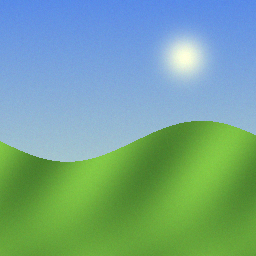
\includegraphics[width=0.31\textwidth]{figures/photo.png}\hfill
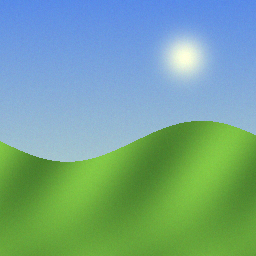
\includegraphics[width=0.31\textwidth]{figures/lsb_full1.png}\hfill
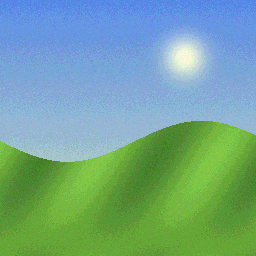
\includegraphics[width=0.31\textwidth]{figures/lsb_full4.png}
\caption{Контейнер (слева) и стегоизображения при полном заполнении одного (в центре)
и четырёх (справа) младших бит}
\label{fig:photo}
\end{figure}

При одном и двух младших битах изменения не видны. При четырёх битах на небе
проступает зернистость: младшие четыре бита составляют до 15 единиц яркости, что уже
сравнимо с плавными переходами цвета.

\textbf{Визуальная атака.} Половина ёмкости заполнялась последовательно, то есть
сообщение занимало верхнюю половину изображения. Для контейнера без шума
(искусственная картинка из тех же форм) плоскость младших бит структурирована, и
область с сообщением видна сразу (рисунок~\ref{fig:attack}); доля совпадающих соседних
бит в верхней половине падает с 0,903 до 0,499 --- уровня случайной
последовательности. У контейнера с шумом сенсора младшие биты случайны уже в
оригинале (0,497), и встраивание их статистику не меняет. Это подтверждает
рекомендацию пособия выбирать в качестве контейнеров отсканированные фотографии.

\begin{figure}[H]
\centering
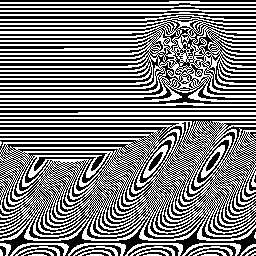
\includegraphics[width=0.31\textwidth]{figures/lsb_plane_flat.png}\hfill

\includegraphics[width=0.31\textwidth]{figures/lsb_plane_flat_stego.png}\hfill

\includegraphics[width=0.31\textwidth]{figures/lsb_plane_photo.png}
\caption{Плоскость младших бит красной составляющей: искусственная картинка до (слева)
и после (в центре) встраивания, фотография с шумом (справа)}
\label{fig:attack}
\end{figure}

\subsection{BPCS-стеганография}

Ёмкость тестового изображения в четырёх младших плоскостях составляющих R, G, B
(12\,288 блоков $8 \times 8$) в зависимости от порога приведена в
таблице~\ref{tab:bpcs}. Она убывает с ростом $\alpha_0$, как и в таблице~7.1 пособия;
при $\alpha_0 = 0{,}3$ ёмкость составила 47,7\,\% объёма изображения против 38\,\% в
пособии, поскольку шумные младшие плоскости тестового изображения почти целиком
шумоподобны.

\begin{table}[H]
\caption{Ёмкость BPCS в зависимости от порога $\alpha_0$}
\label{tab:bpcs}
\centering
\begin{tabular}{crrr}
\toprule
$\alpha_0$ & Шумоподобных блоков & Ёмкость, байт & Доля объёма \\
\midrule
0,20 & 12\,257 & 96\,519 & 49,1\,\% \\
0,25 & 12\,162 & 95\,771 & 48,7\,\% \\
0,30 & 11\,915 & 93\,826 & 47,7\,\% \\
0,35 & 11\,433 & 90\,030 & 45,8\,\% \\
0,40 & 10\,690 & 84\,179 & 42,8\,\% \\
0,45 & 8\,637 & 68\,012 & 34,6\,\% \\
0,50 & 5\,147 & 40\,528 & 20,6\,\% \\
\bottomrule
\end{tabular}
\end{table}

Сообщение длиной 104 байта заняло 14 блоков, один из них записан конъюнкцией. При
полном заполнении (93\,826 байт) конъюнкций потребовали лишь 20 блоков из 11\,915:
блоки текста, закодированного в UTF-8, сами по себе достаточно сложны. PSNR при этом
32,0~дБ, и на однотонном небе видны полосы (рисунок~\ref{fig:bpcs}): четвёртая
плоскость соответствует 8 единицам яркости, а её блоки на плавном градиенте ещё
проходят порог сложности из-за шума. Для скрытности следует ограничиваться двумя-тремя
младшими плоскостями или повышать $\alpha_0$ в старших плоскостях.

\begin{figure}[H]
\centering
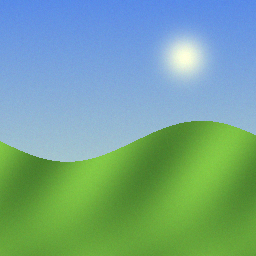
\includegraphics[width=0.38\textwidth]{figures/photo.png}\qquad
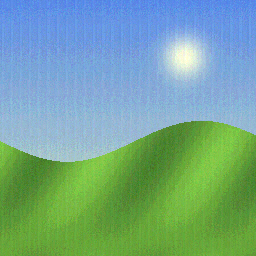
\includegraphics[width=0.38\textwidth]{figures/bpcs_full.png}
\caption{Контейнер и стегоизображение BPCS при полном заполнении четырёх плоскостей,
$\alpha_0 = 0{,}3$}
\label{fig:bpcs}
\end{figure}

\subsection{Метод CPT и его модификация}

Бинарное изображение $128 \times 96$ (рисунок~\ref{fig:cpt}) разбивалось на блоки $4
\times 4$ с $r = 4$, матрицы $K$ и $W$ порождались стегоключом. Сообщение длиной 104
байта заняло 212 блоков и изменило 250 бит (1,18 на блок, не более двух в каждом) в
обоих вариантах метода.

\begin{figure}[H]
\centering

\includegraphics[width=0.48\textwidth]{figures/cpt_basic.png}\hfill

\includegraphics[width=0.48\textwidth]{figures/cpt_modified.png}
\caption{Изменённые биты (красным) при встраивании базовым (слева) и модифицированным
(справа) методом CPT}
\label{fig:cpt}
\end{figure}

В блоках, содержащих границу цветов, модифицированный метод поместил на границу 77\,\%
изменений против 49\,\% у базового, а число изолированных точек уменьшилось с 187 до
163. На белом фоне выигрыша нет: в одноцветном блоке все биты равноудалены от границы,
и любая инверсия создаёт точку. Поэтому для встраивания в бинарные изображения
предпочтительны контейнеры с большим числом границ --- отсканированный текст, чертежи,
подписи, --- а одноцветные блоки следует пропускать.

\subsection{Самопроверка}

Сорок случайных сообщений из русских и латинских букв, цифр и знаков препинания
прошли через все методы со случайными параметрами: LSB с 1--3 младшими битами и
случайным ключом, BPCS со случайным $\alpha_0$, CPT со случайными размером блока
($4 \times 4$, $3 \times 4$, $6 \times 6$, $8 \times 8$), $r$ и ключом, все шесть
текстовых методов. Все сообщения извлечены без искажений, в каждом блоке CPT изменено
не более двух бит.

\listingcaption{Вывод программы}{lst:demo}
\VerbatimInput[fontsize=\scriptsize, frame=single]{listings/demo_output.txt}

\section{Анализ методов}

\subsection{Ёмкость и скрытность}

Методы образуют ряд от малой ёмкости к большой, и скрытность в нём убывает.
Синтаксические текстовые методы вмещают около бита на слово и разрушаются любым
переформатированием; лексические сохраняют сообщение при перепечатке, но требуют
словаря и меняют стиль текста. Метод LSB с одним битом вмещает $1/8$ изображения и
незаметен на шумных фотографиях, но обнаруживается визуальной атакой на искусственных
картинках. BPCS вмещает почти половину изображения, поскольку выбирает для замены
только шумоподобные участки, однако при заполнении старших плоскостей становится
заметен. CPT для бинарных изображений вмещает лишь $r$ бит на блок, зато меняет не
более двух бит в блоке.

\subsection{Стегоанализ}

Атака на основе знания алгоритма читает сообщение без ключа: в методах LSB и BPCS без
стегоключа данные лежат в предсказуемых местах. Ключевая перестановка в LSB и
матрицы $K$, $W$ в CPT заставляют противника перебирать ключи. Статистическая атака
обнаруживает не содержимое, а факт встраивания: младшие биты заполненного контейнера
равновероятны, а в естественном изображении нет; на этом основаны атаки хи-квадрат и
RS-анализ для LSB. Поэтому сообщение следует предварительно шифровать (тогда его биты
неотличимы от случайных) и заполнять контейнер не полностью.

\subsection{Устойчивость к преобразованиям}

Все реализованные методы хрупкие: сообщение не переживает сжатия с потерями (JPEG),
масштабирования, фильтрации или печати и сканирования. Для скрытой переписки это
допустимо, но для водяных знаков, защищающих авторские права, требуется устойчивость,
которую обеспечивают методы встраивания в частотную область (коэффициенты DCT или
вейвлет-преобразования) с избыточным кодированием. Хрупкие водяные знаки, напротив,
полезны для контроля целостности: любое изменение изображения разрушает метку и тем
самым обнаруживается.

\subsection{Стеганография в защите авторских прав}

Водяной знак, встроенный методом этой работы, подтверждает авторство, если автор
может извлечь его своим ключом из спорной копии. Отпечаток пальца --- уникальный
идентификатор покупателя в каждой копии --- позволяет найти источник утечки, как в
случае с документом кабинета министров Великобритании 1981~года, описанным в пособии.
Стеганографическая метка дополняет цифровую подпись из лабораторной работы №3: подпись
доказывает целостность и авторство, но легко отделяется от файла, а встроенная метка
остаётся в самом произведении и сопровождает каждую его копию.

\sectioncenter{Заключение}

В ходе лабораторной работы изучены методы стеганографии главы~7 пособия и реализована
программа, выполняющая встраивание и извлечение сообщений шестью текстовыми методами,
методами LSB и BPCS для цветных изображений и методом CPT с модификацией для
бинарных изображений. Программа имеет интерфейс командной строки и графическое окно с
пошаговым разбором и использует только стандартную библиотеку Python, включая
собственные чтение и запись PNG и BMP. Все числовые примеры пособия воспроизведены
точно: <<кОмПьютер>>, выбор синонима <<predilection>>, 5 бит смешанного основания
против 4, предложение мимикрии для кода 1010, встраивание символа A методом LSB,
меры сложности $\alpha$ и $\beta$ эталонных блоков, множества $S_1, \ldots, S_7$ и
изменённый бит (2,4) метода CPT.

Эксперименты показали, что ёмкость покупается заметностью: LSB при четырёх битах
вмещает 50\,\% изображения при PSNR 33~дБ и даёт видимую зернистость, BPCS при
пороге 0,3 вмещает 47,7\,\%, но при заполнении четырёх плоскостей оставляет полосы на
однотонных участках. Решающим оказался выбор контейнера: на искусственной картинке
сообщение в младших битах видно на плоскости LSB, а на фотографии с шумом сенсора
статистика младших бит после встраивания не меняется. Модифицированный метод CPT
переносит изменения на границы цветов (77\,\% против 49\,\%), но бессилен в
одноцветных блоках.

\sectioncenter{Список использованных источников}

\begin{enumerate}
\item Ярмолик, В.~Н. Криптография, стеганография и охрана авторского права /
В.~Н.~Ярмолик, С.~С.~Портянко, С.~В.~Ярмолик. --- Минск: Издательский центр БГУ,
2007. --- Гл.~7.
\item Грибунин, В.~Г. Цифровая стеганография / В.~Г.~Грибунин, И.~Н.~Оков,
И.~В.~Туринцев. --- М.: СОЛОН-Пресс, 2002. --- 272~с.
\item Kawaguchi, E. Principle and applications of BPCS-steganography / E.~Kawaguchi,
R.~O.~Eason // Proc. SPIE Multimedia Systems and Applications. --- 1998. ---
Vol.~3528. --- P.~464--473.
\item Tseng, Y.-C. A secure data hiding scheme for binary images / Y.-C.~Tseng,
Y.-Y.~Chen, H.-K.~Pan // IEEE Transactions on Communications. --- 2002. --- Vol.~50,
No.~8. --- P.~1227--1231.
\item Fridrich, J. Steganography in digital media: principles, algorithms, and
applications / J.~Fridrich. --- Cambridge: Cambridge University Press, 2009. ---
437~p.
\end{enumerate}

\end{document}
